\documentclass{standalone}
\usepackage[dvipsnames,svgnames,x11names]{xcolor}
\usepackage{tikz}
\usepackage{pgfplots}
\pgfplotsset{compat = 1.12}
\usepackage[
  group-separator={,},
  exponent-product=\cdot,
  binary-units = true,
]{siunitx}
\usepackage{../thesismath}
\begin{document}
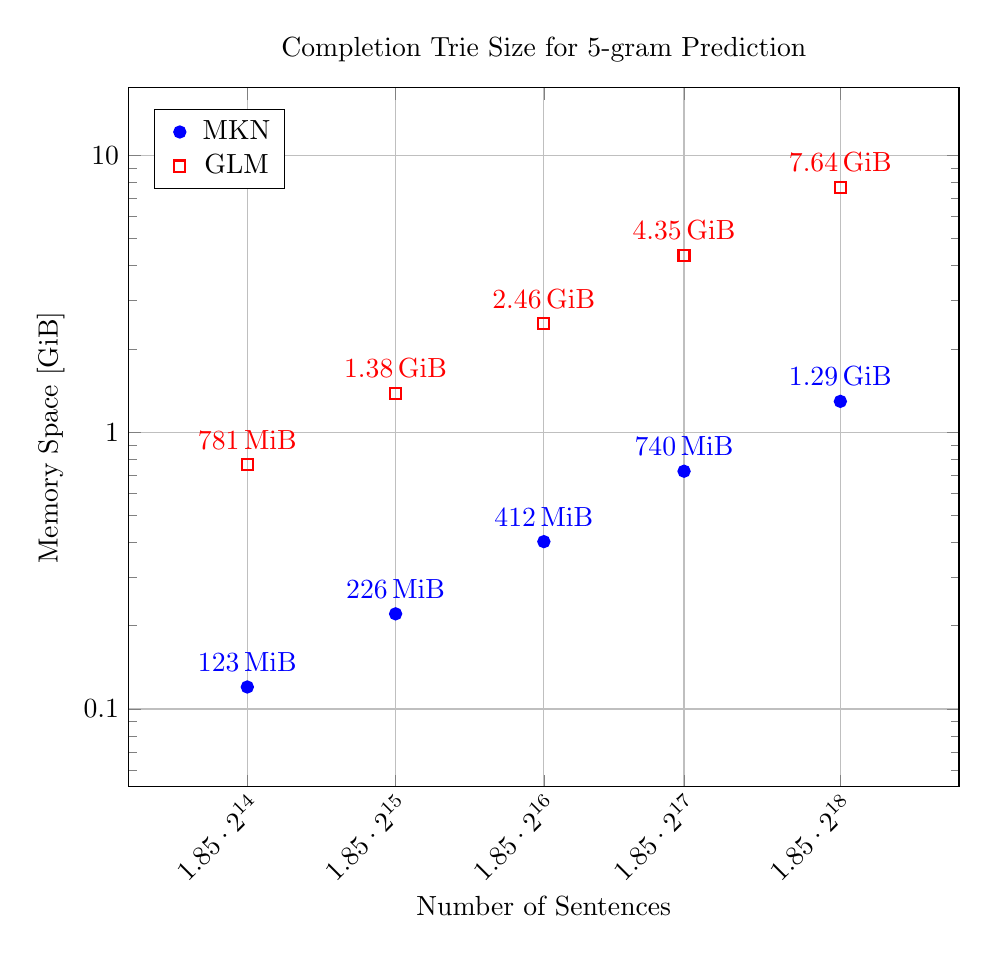
\begin{tikzpicture}[baseline]

\pgfplotscreateplotcyclelist{mkn_glm}{%
  blue,  mark size=2, mark=*,      thick,\\%
  red,   mark size=2, mark=square, thick,\\%
}

\pgfplotsset{
  legend style = {
    legend image code/.code = {
      \draw[only marks]
        plot coordinates {
          (0.3cm,0cm)
        };
      \node at (0.15cm, 0cm) {};
      \node at (0.45cm, 0cm) {};
    },
  },
}

\sisetup{exponent-base = 2}
\begin{axis}[
  title = {Completion Trie Size for $5$-gram Prediction},
  xlabel = {Number of Sentences},
  xmode = log,
  xtick       = {        30400,         60801,        121602,        234204,        486409},
  xticklabels = {\num{1.85e14}, \num{1.85e15}, \num{1.85e16}, \num{1.85e17}, \num{1.85e18}},
  xticklabel style = {
    inner sep = 1pt,
    anchor = north east,
    rotate = 45,
  },
  ylabel = {Memory Space [\si{\gibi\byte}]},
  %ytick = {100, 1000, 10000},
  %yticklabels = {\num{0.1}, \num{1.0}, \num{10.0}},
  ymode = log,
  log ticks with fixed point,
  %ymin = 0,
  minor y tick num = 4,
  grid = major,
  enlargelimits = 0.2,
  cycle list name = mkn_glm,
  legend entries = {{MKN}, {GLM}},
  legend pos = north west,
  width = \textwidth,
]

% MKN
\addplot+[
  only marks,
] table [y expr = \thisrow{mb}/1024] {
  n      mb
   30400  123
   60801  226
  121602  412
  234204  740
  486409 1323
};

\node [blue, yshift = 0.5ex] at ({axis cs: 30400, 0.12}) [above] {\SI{ 123}{\mebi\byte}};
\node [blue, yshift = 0.5ex] at ({axis cs: 60801, 0.22}) [above] {\SI{ 226}{\mebi\byte}};
\node [blue, yshift = 0.5ex] at ({axis cs:121602, 0.40}) [above] {\SI{ 412}{\mebi\byte}};
\node [blue, yshift = 0.5ex] at ({axis cs:234204, 0.72}) [above] {\SI{ 740}{\mebi\byte}};
\node [blue, yshift = 0.5ex] at ({axis cs:486409, 1.29}) [above] {\SI{1.29}{\gibi\byte}};

% GLM
\addplot+[
  only marks,
] table [y expr = \thisrow{mb}/1024] {
  n      mb
   30400  781
   60801 1412
  121602 2524
  234204 4458
  486409 7821
};

\node [ red, yshift = 0.5ex] at ({axis cs: 30400, 0.76}) [above] {\SI{ 781}{\mebi\byte}};
\node [ red, yshift = 0.5ex] at ({axis cs: 60801, 1.38}) [above] {\SI{1.38}{\gibi\byte}};
\node [ red, yshift = 0.5ex] at ({axis cs:121602, 2.46}) [above] {\SI{2.46}{\gibi\byte}};
\node [ red, yshift = 0.5ex] at ({axis cs:234204, 4.35}) [above] {\SI{4.35}{\gibi\byte}};
\node [ red, yshift = 0.5ex] at ({axis cs:486409, 7.64}) [above] {\SI{7.64}{\gibi\byte}};

%\addplot [blue, domain=30400:486409, samples=100]
%  {1.7e-5*x^0.857};
%\addplot [ red, domain=30400:486409, samples=100]
%  {1.4e-4*x^0.832};

\end{axis}

\end{tikzpicture}
\end{document}
